% -*- coding: UTF-8 -*-
% vim: autoindent expandtab tabstop=4 sw=4 sts=4 filetype=tex
% chktex-file 27 - disable warning about missing include files

\section{Oberflächen}
\label{sec:surfaces}

Sofern nicht anders vermerkt, basiert der folgende Abschnitt
auf~\cite{division_introduction_1996}[S. 1 ff] sowie
auf~\cite{glassner_introduction_1989}[S. 79 bis 115].\\
\\
Um in Computergrafiken überhaupt etwas darstellen zu können, muss erst einmal
definiert werden, was dargestellt werden soll. Häufig orientiert sich die
Computergrafik dabei an der realen Welt.  In der realen Welt haben Oberlächen
von Objekten häufig keine starken Übergänge (Kanten) sondern sind eher von
glatter Natur~\cite{foley_computer_1996}[S. 471].\\
\\
Die Darstellung von Kurven und Oberflächen führt zu zwei Fällen: Modellierung
von bestehenden Objekten und Modellierung von Grund auf.\\
\\
Zur Modellierung von Oberflächen werden hauptsächlich zwei Techniken verwendet:
Parametrische Modellierung und implizite Modellierung.\\
\\
Bei der parametrischen Darstellung wird eine Oberfläche üblicherweise als
eine Menge von Punkten definiert, so zum Beispiel:

\begin{gather}\label{eq:surface_parametric}
    \bm{p}(s, t) = (x(s, t), y(s, t), z(s, t))
\end{gather}

So kann eine Kugel mittels sphärischen Koordinaten wie
folgt parametrisch dargestellt werden:

\begin{align}\label{eq:sphere_parametric}
    x(s, t) &= r \cdot \cos(s) \cdot \sin(t) \\
    y(s, t) &= r \cdot \sin(s) \cdot \sin(t) \\
    z(s, t) &= r \cdot \cos(t)
\end{align}

Wobei $r$ der Radius der Kugel, $s$ der Azimutwinkel $\in [0, 2\pi]$ und
$t$ der Polarwinkel $\in [0, \pi]$.

Bei der impliziten Darstellung wird eine Oberfläche üblicherweise als Kontur
einer Funktion mit Wert 0 definiert, so zum Beispiel:

\begin{gather}\label{eq:surface_implicit}
    f(\bm{p}) = f(x, y, z) = 0
\end{gather}

Wobei $\bm{p}$ ein Punkt $(x, y, z)$ auf der Oberfläche, welche durch die Funktion
$f$ beschrieben wird, ist.

Am Beispiel einer Kugel:

\begin{align}\label{eq:sphere_implicit}
    f(\bm{p}, r) = f(x, y, z, r) &= 0 \\
    f(\bm{p}, r) = \bm{p}^{2} - r^{2} &= 0 \\
    f(\bm{p}, r) = x^{2} + y^{2} + z^{2} - r^{2} &= 0
\end{align}

Wobei $\bm{p}$ ein Punkt $(x, y, z)$ auf der Oberfläche, welche durch die Funktion
$f$ beschrieben wird, und $r$ der Radius der Kugel ist.~\cite{glassner_introduction_1989}[S. 91]

Die parametrische Darstellung bringt Vorteile wie die Unabhängigkeit von einem
Koordinatensystem oder eine effiziente Berechnung von Punkten auf einer
Oberfläche. Die implizite Darstellung erlaubt hingegen eine grössere
Einflussnahme aus mathematischer Sicht und ist daher sehr nützlich für
Operationen wie Biegung, Vermischung, Schnitte (Intersektion) oder Bool'sche
Operationen.

\subsection{Implizite Oberflächen}
\label{subsec:implicit_surfaces}

Wie in Gleichung~\ref{eq:surface_parametric} beschrieben, ist eine implizite
Oberfläche gemäss~\cite{hart_ray_1993}[S. 1] als Funktion $ f(\bm{x}) =
\mathbb{R}^{3} \to \mathbb{R} $ definiert.  Es wird also jedem Punkt einer
Menge $ \bm{p} \in \mathbb{R}^{3} $ ein skalarer Wert $ s \in \mathbb{R} $
zugewiesen. Dabei besteht die Oberfläche aus der Punktemenge $ \bm{x} \equiv
(x, y, z) \in \mathbb{R}^{3} $.\\
\\
Angenommen $ \bm{A} $ ist ein geschlossener Festkörper, welcher durch die
Funktion $f$ beschrieben wird, dann kann gemäss~\cite{hart_ray_1993} Folgendes
angenommen werden:

\begin{align} \label{eq:surface_implicit_condition}
    x \in \overset{\circ}{\bm{A}} \Leftrightarrow f(\bm{x}) &< 0 \\
    x \in \partial \bm{A}         \Leftrightarrow f(\bm{x}) &= 0 \\
    x \in \mathbb{R}^{3} - \bm{A} \Leftrightarrow f(\bm{x}) &> 0
\end{align}

Dies bedeutet, dass sich ein Punkt $\bm{x}$:
\begin{itemize}
    \item $\overset{\circ}{\bm{A}}$, genau dann \textit{innerhalb} des Körpers
        $\bm{A}$ befindet, wenn die implizite Funktion $f(\bm{x})$ \textit{negativ}
        ist
    \item $\partial{\bm{A}}$, genau dann \textit{auf der Oberfläche} des
        Körpers $\bm{A}$ befindet, wenn die implizite Funktion $f(\bm{x})$
        \textit{0} ist
    \item $\mathbb{R}^{3} - \bm{A}$, \textit{nicht in oder auf} dem Körper
        $\bm{A}$ befindet, wenn die implizite Funktion $f(\bm{x})$ \textit{positiv}
        ist
\end{itemize}

Dies gilt, da es sich bei $ \bm{x} $ um eine Punktemenge mit topologischer
Struktur handelt.\\
\\
Gemäss~\cite{division_introduction_1996} finden hauptsächlich drei Methoden
Anwendung zur Beschreibung impliziter Oberflächen: algebraische Oberflächen,
Blobby-Objekte sowie die funktionale Repräsentation.~\cite{hart_sphere_1994}
gibt jedoch an, dass die gebräuchlichste Form von impliziten Oberflächen die
algebraischen Oberflächen sind. Diese werden implizit durch polynomiale
Funktionen definiert.\\

\subsubsection{Algebraische und geometrische implizite Oberflächen}
\label{ssubsec:implicit_surfaces_algebraic_geometric}

Ein Beispiel für eine algebraische Oberfläche ist die Beschreibung der
Einheitskugel anhand einer impliziten algebraischen Gleichung zweiten Grades:

\begin{gather} \label{eq:surface_immplicit_algebraic}
    x^{2} + y^{2} + z^{2} - 1 = 0
\end{gather}

Wobei es sich bei dem letzten Parameter um den Radius $r$ handelt, welcher ---
bedingt durch die Einheitskugel --- den Wert 1 hat.

Wie~\cite{division_introduction_1996} schreibt, handelt es sich bei impliziten
Oberflächen, welche durch eine polynomiale Funktion zweiten Grades beschrieben
werden, um quadrische implizite Oberflächen.

\cite{hart_sphere_1994} gibt weiter an, dass --- unter Nuztung einer Metrik ---
die Einheitskugel durch die implizite Gleichung

\begin{gather} \label{eq:surface_immplicit_geometric}
    \|\bm{x}\| - 1 = 0
\end{gather}

beschrieben werden kann, was unter Anwendung der allgemeinen
Form~\ref{eq:surface_implicit} einer impliziten
Gleichung~\ref{eq:surface_implicit} zu folgender Gleichung führt:

\begin{gather}\label{eq:surface_implicit_sphere}
    f(\bm{x}) = \|\bm{x}\| - 1
\end{gather}


Dabei ist $\|\bm{x}\|$ als euklidische Metrik definiert und entspricht ${(x^{2} + y^{2} + z^{2})}^{1 \over 2}$.\\
\\
Die Gleichung~\ref{eq:surface_immplicit_algebraic} gibt die algebraische
Distanz zurück, Gleichung~\ref{eq:surface_immplicit_geometric} gibt die
geometrische Distanz zurück.\\

\subsubsection{Distanzfunktionen}
\label{ssubsec:distance_functions}

Gemäss~\cite{hart_sphere_1994} wird die geometrische Darstellung von
quadrischen Oberflächen bevorzugt, da deren Parameter unabhängig von
Koordinaten sind, sie robuster und intuitiver sind. Es handelt sich dabei um
eine \textbf{Distanzfunktion}.\\
\\
Wie anfangs erwähnt, definiert~\cite{hart_sphere_1994} die allgemeine Form zur
Beschreibung bzw. Darstellung von impliziter Oberflächen als Zuweisung von
Punkten zu einem skalaren Wert: $ f : \mathbb{R}^{n} \to \mathbb{R} $.\\
\\
Unter Anwendung der unter~\ref{eq:surface_implicit_condition} definierten
Bedingungen kann geschlossen werden, dass eine Menge von Punkten $A$ existiert,
welche Teil von $\mathbb{R}^{n}$, also $A \subset \mathbb{R}^{n}$ ist. Dies heisst, dass alle Punkte in $A$ die folgende Bedingung erfüllen:

\begin{gather}
    A = \{ x : f(x) \leq 0 \}
\end{gather}

\cite{hart_sphere_1994} liefert zwei Definition, welche der Beschreibung von Distanzfunktionen dienen:

\theoremstyle{definition}
\begin{definition}{\label{theo:point_to_set_distance}
    \textit{Point-to-set distance}}\\
    Die Distanz eines Punktes zu einer Menge von Punkten definiert die Distanz
    eines Punktes $ \bm{x} \in \mathbb{R}^{3} $ zu einer Menge von Punkten $A
    \subset \mathbb{R}^{3}$ als Distanz von $\bm{x}$ zum nähesten Punkt in $A$:

    \begin{gather}
        d(\bm{x}, \bm{A}) = \min_{\substack{\bm{y} \in \bm{A}}}(\|\bm{x} - \bm{y}\|)
    \end{gather}
\end{definition}

\theoremstyle{definition}
\begin{definition}{\label{theo:signed_distnace_bound}
    \textit{Signed distance bound}}\\ 
    Eine Funktion $ f : \mathbb{R}^{3} \to \mathbb{R} $ ist eine
    vorzeichenabhängige Obergrenze ihrer impliziten Oberfläche $ f^{-1}(0)$,
    wenn gilt:

    \begin{gather}\label{eq:signed_distnace_bound}
        |f(\bm{x})| \leq d(\bm{x}, f^{-1}(0))
    \end{gather}
\end{definition}

Wenn die Gleichung~\ref{eq:signed_distnace_bound} für eine Funktion $f$ gilt,
dann ist $f$ eine \textit{vorzeichenabhängige Distanzfunktion (signed distance
    function)}.

\subsubsection{Distanzfelder (distance fields)}
\label{ssubsec:distance_fields}

\todo[inline]{Introduce distance fields?}

Sofern nicht anders vermerkt, basiert der folgende Abschnitt
auf~\cite{jones_3d_2006}.

Bei einem Distanzfeld handelt es sich um eine Repräsentation respektive eine
Datenstruktur, bei welcher von jedem Punkt aus die geringste Distanz zu
einem beliebigen Objekt der Domäne bekannt ist.

Zusätzlich zu der Distanz können aus einem Distanzfeld andere Parameter
wie beispielswiese die Richtung einer Oberfläche abgeleitet werden.

Handelt es sich bei einem Distanzfeld um ein vorzeichenbehaftetes
Distanzfeld, so kann bei jedem Punkt bestimmt werden, ob sich dieser
innerhalb, ausserhalb oder genau auf einem Objekt befindet. Dies verhält
sich analog zu Abschnitt~\ref{subsec:implicit_surfaces}.

Distanzfelder bilden somit die Grundlage der Algorithmen zur Darstellung
von impliziten Oberflächen. Siehe dazu auch
Kapitel~\ref{sec:rendering_implicit_surfaces}. Die unter
Abschnitt~\ref{ssubsec:distance_functions} genannte~\textit{Point-to-set
    distance}-Funktion  liefert bereits die näheste Distanz zu einer
Menge von Punkten und somit auch zu Objekten auseghend von einem Punkt
der Domäne.

\begin{figure}[H]
    \centering
    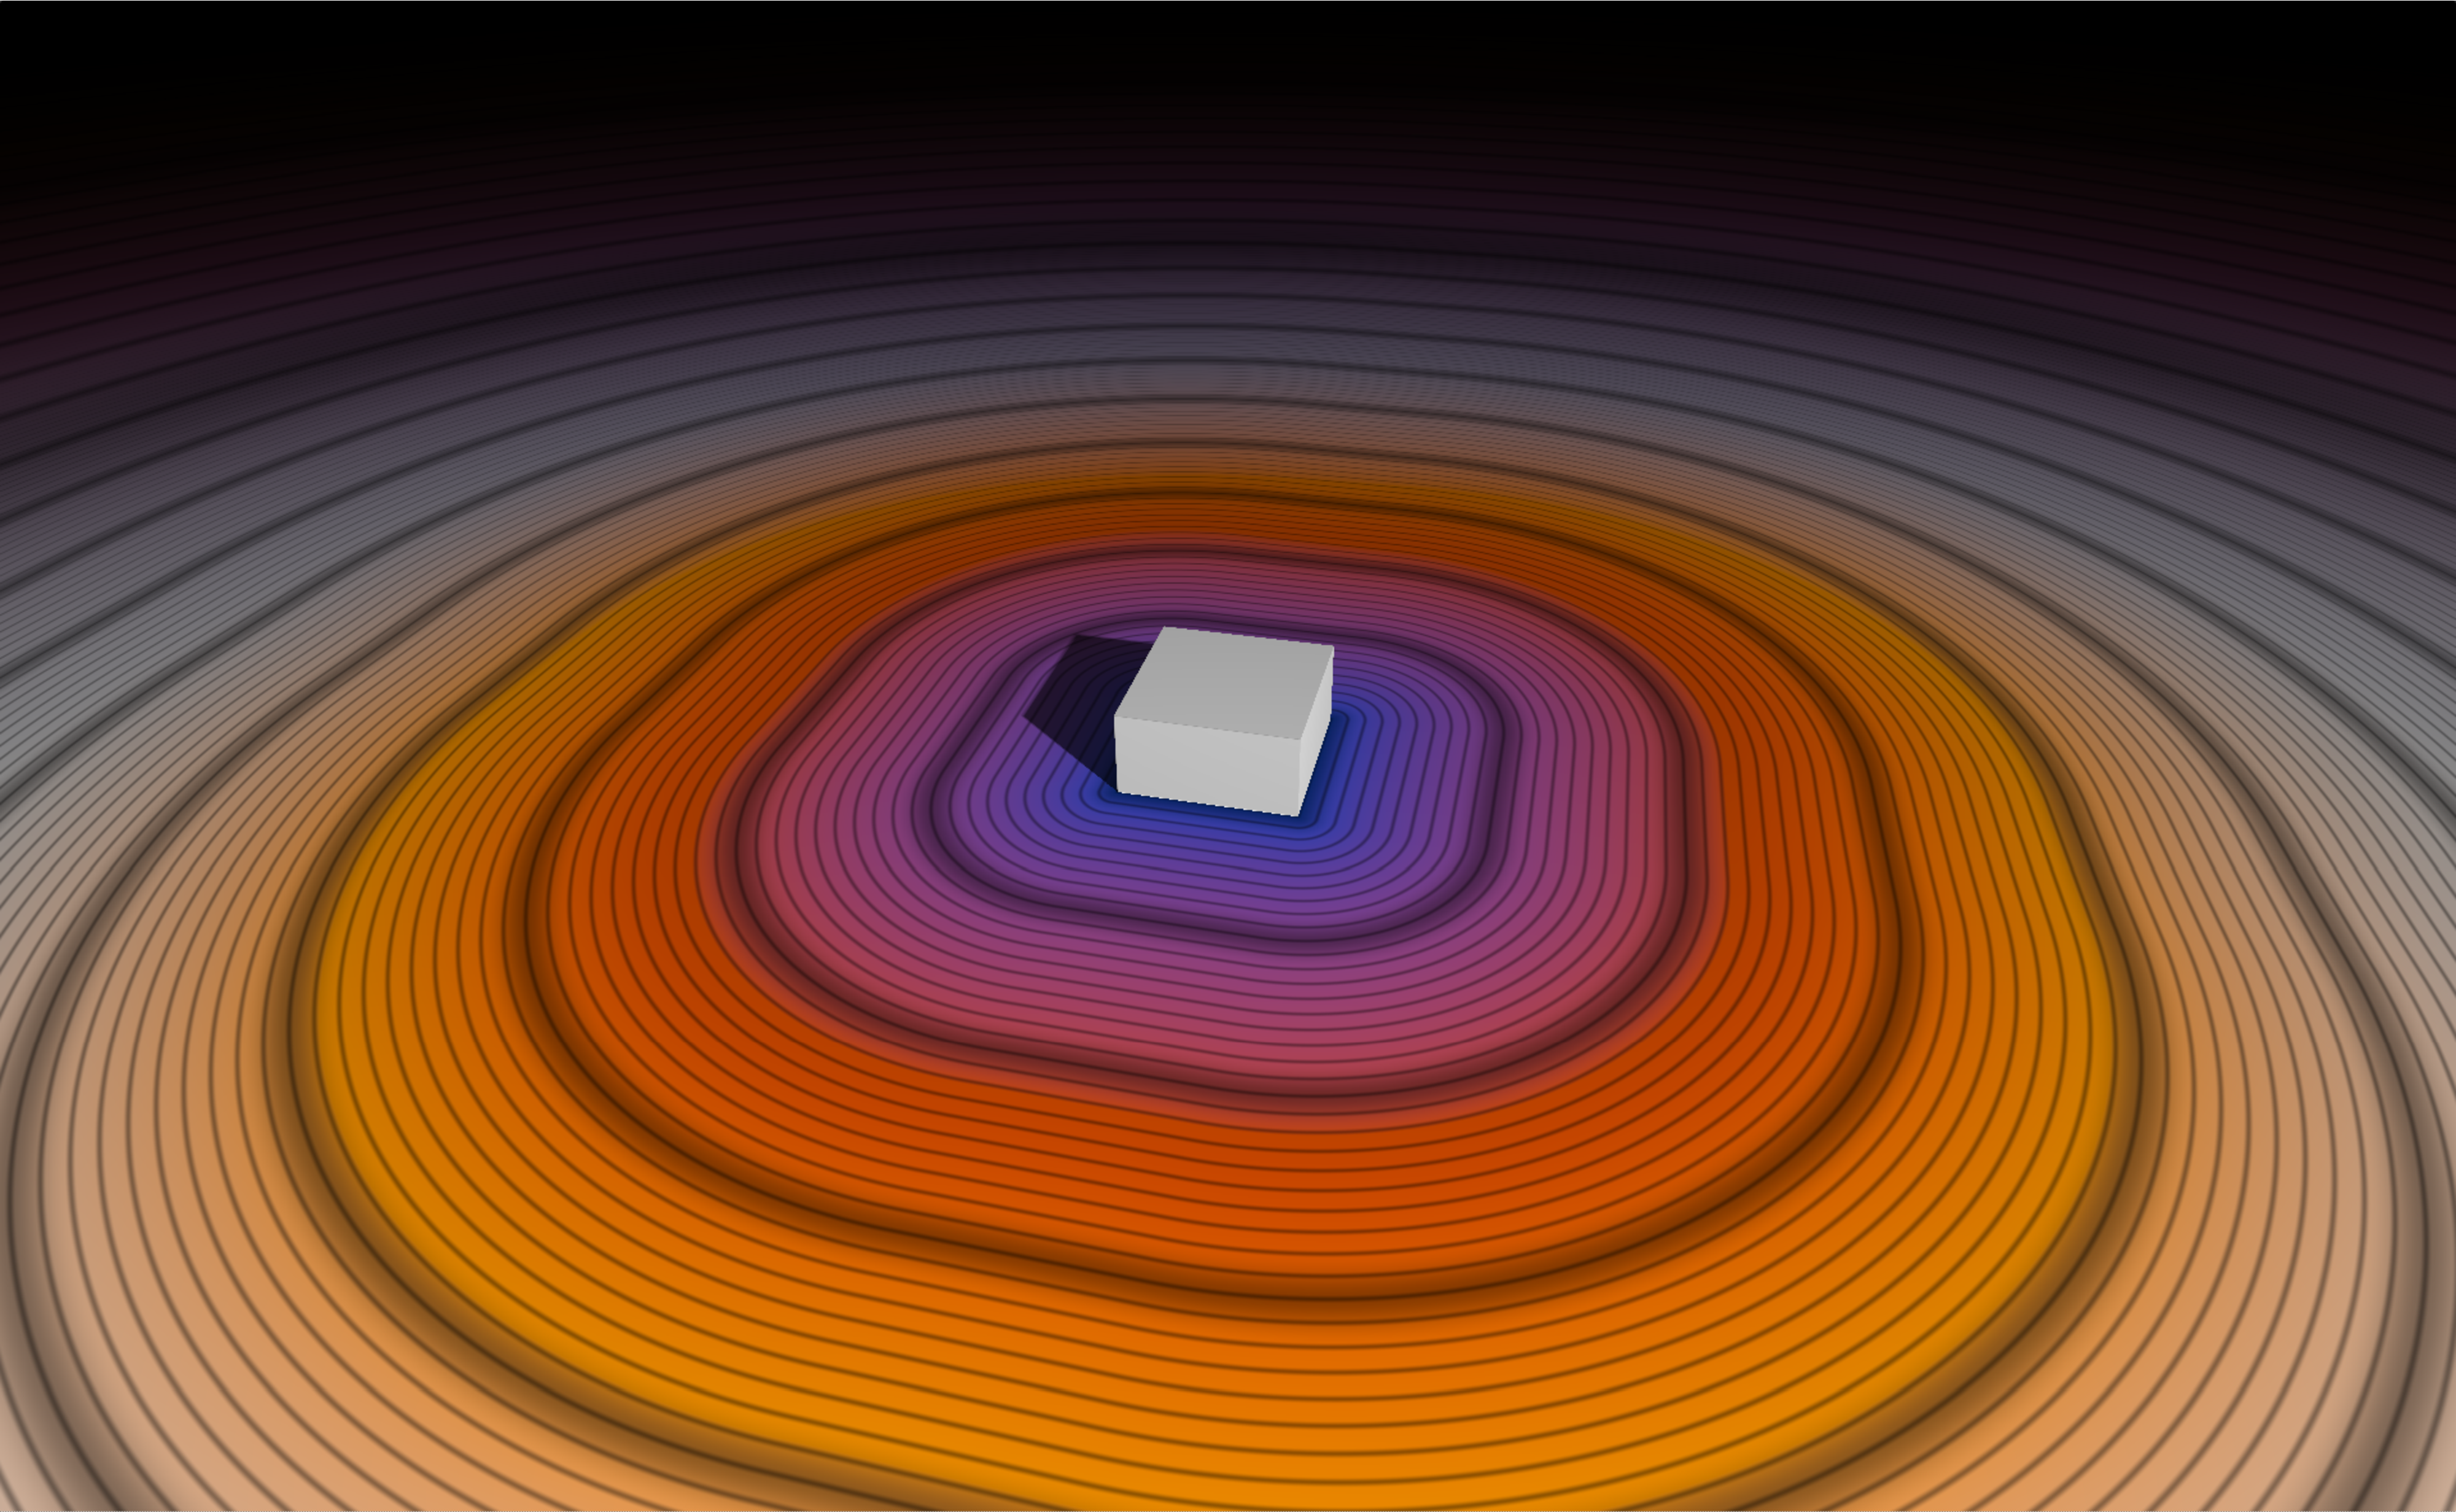
\includegraphics[width=1.0\textwidth]{img/distance_field.pdf}
    \caption{Darstellung des Dinstanzfeldes einer dreidimensionalen
        Szene anhand Farbwerten\protect\footnotemark}\label{
        fig:distance_field_illustration}
\end{figure}
\footnotetext{Eigene Darstellung}
